%
% latex-sample.tex
%
% This LaTeX source file provides a template for a typical research paper.
%

%
% Use the standard article template.
%
\documentclass{article}

\usepackage{geometry}
\geometry{letterpaper}

\usepackage{pgfplots}
\usepackage{cite}
\usepackage{doc}
\usepackage{url}
\usepackage{graphicx}
\usepackage{aaai}
\usepackage{amsmath}
\usepackage{epstopdf}
\usepackage{hyperref}
\usepackage{caption}

\title{Energy Disaggregation}
\author{Henry Agsten, Jacob Denson, Jesse Huard, Isabel McCarten, Morgan Redshaw}

\date{}

\begin{document}

\maketitle

\begin{abstract}
Energy disaggregation is the process of generating estimates of per-appliance power consumption from aggregated power consumption data showing the power usage of an entire building. This paper takes the unusual approach of trying to disaggregate power consumption using only binary indicators of whether applainces were on or off in the training phase rather than the actual disaggregate data. Two preprocessing methods on the aggregated power consumption and the binary indicators were used to generate an approximation of the disaggregated, per-device power consumption which was used to train a denoising autoencoder, a type of neural network. We present a comparison of the two preprocessing methods and the performance of the neural nework when trained on data generated from them or the actual disaggregated data with the goal of demonstrating whether the loss of information from using just the indicators seriously affects the performance of the neural network.

\end{abstract}

%TODO: Do we assume that are either ON or OFF, or that they can have multiple levels?
	%NOTE: another paper assumed that 'all appliances that have more than two states (e.g., on and off) will produce events that can be explained by two-state appliances'
%TODO: Outline where we got the data from

\section{Introduction}

Energy disaggregation, or non-intrusive load-monitoring (NILM), is the problem of estimating a household's individual appliance energy consumption given measurements from a single sensor which records the aggregate power consumption of the household over time.
While measuring the power draw of each device in a home directly yields more accurate results than machine learned techniques, it usually involves either expensive instrumentation of the devices we wish to measure the energy consumption of or intrusion into the home in order to set up power monitoring hardware.
Both situations are undesirable for the homeowner, so instead NILM makes use of already existing infrastructure combined with machine learned techniques, in order to provide an estimate of device energy consumption.

Having access to disaggregated energy consumption is useful to homeowners, as studies have shown that when presented with this information, they are more motivated to reduce their energy consumption \cite{Darby}.
Additionally, this information can be used to identify devices in a home which have become faulty and are in need of repair.
When a device breaks, changes in its energy consumption patterns can be detected by an automated system, allowing the homeowner to be notified that the device needs servicing.

Most existing machine learning methodologies for NILM are trained using data from households which have been instrumented to record the power consumption of each device separately, in addition to the aggregate household power usage \cite{Kelly, Cicchetti}.
However, as noted above, this instrumentation is expensive and makes it difficult to gather new data, with most existing datasets being limited to recording from only a small number of homes \cite{Redd, Kelly2}.
This lack of data from many homes has the effect of making it difficult to see how well current NILM algorithms generalize to unseen homes, and can be problematic with algorithms which require large amounts of data, such as deep neural network architectures \cite{Kelly}.

The authors of this paper believe it is valuable to explore machine learning techniques which use only the binary on-off indicators of household devices during training, as opposed to the raw power consumption of each device.
With the rise of the ``Internet of Things'', it seems reasonable that in the near future, network-enabled home appliances will be able to report their periods of activity to a remote data analytics platform \cite{Gubbi}.
Once collected, these binary indicators can be used along with the aggregate power consumption data to find an approximation to the power draw of each individual device in the household.
These binary indicators forgo the need for expensive instrumentation in each device to monitor power usage, meaning that training data can be continuously collected by an automated system operating at a large scale.

In this paper, we investigate several different pre-processing algorithms for approximating single device power usage given a household's aggregate power usage and binary on-off indicators for each device in the home.
To evaluate the effect of our pre-processing compared to state-of-the-art NILM algorithms which use single device power consumption, we use a previously-identified neural network architecture based on denoising auto-encoders \cite{Kelly}.
For each device network, we trained separately on the raw device power usage and the approximate power usage obtained by each pre-processing algorithm.
We then compared the output of each device network to a hold-out set, in order determine the performance impact of our pre-processing algorithms on the NILM task.

\section{Related Work}

%NOTE: Should focus on research relevant to ours. Don't know how much there is.
%TODO: Should also outline one or two unsupervised approaches.

During our literature review, we found no other NILM studies which used only the binary on-off indicators of each device along with the aggregated power usage.
%TODO: Cite all of these
There have been supervised approaches using the disaggregated energy\cite{Kelly} or energy signatures \cite{Parson} for each device.
Some unsupervised approaches also exist that only use the aggregated energy of the overall house \cite{Kolter}.
%TODO: Mention something about related approaches or similar ideas?

\subsection{Hidden Markov Models}

Hidden Markov models are one of the main categories of methods used for energy disaggregation.
For example, \cite{Kolter} used one hidden Markov model per device to describe its power consumption, in order to determine which times the device was active at.
Kolter's algorithm finds periods of device activity, and clusters similar periods to build one hidden Markov model per device \cite{Kolter}.
Unfortunately the algorithm to find these periods is not described in detail, though it seems to find them by looking for intervals when only one device is active.
For some devices, \cite{Kolter} claims to reach precision values of over 90\%, but since the recall values are not given it is hard to judge these results.

In contrast to this completely unsupervised approach, Parson \cite{Parson} starts with knowledge about the general device type and produces a generic model for each device, which is then fitted to the actual device.
The generic and fitted models are difference hidden Markov models \cite{Kolter} which have a second observation sequence representing the difference in power consumption between two time steps.
The algorithm's biggest benefit is that it identifies the devices without the need for manual labelingn \cite{Parson}, unlike most unsupervised methods in which the output disaggregated power consumption for some device has to be manually matched with an existing device.
The algorithm also has the advantage that it does not require the assumption that the number of devices in the house is known.
For devices with clearly distinguished patterns (e.g. fridges) Parson reaches F-scores up to 85\%, while achieving results under 20\% for unstable devices (e.g. microwaves).
Even though his allocation of generic models and minute-wise measurements did not seem useful for our approach, Parson's work led us to the REDD-dataset and to the idea of looking for timesteps when only one device changes its activity status.


%TODO: Citations for this

%Weiss \cite{Weiss} presumes the power consumption as a sequence of piecewise constant consumption levels those differences 
%describe the typical consumption pattern of a distinct device. They identify devices by checking for characteristic 
%differences 
%between consumption changes and look for the most similar device pattern via neareast neighbor calculation. Since they get remarkable 
%F-scores of 80\% and higher for some devices although the strong assumption we also have a look on signal for which this assumption holds.

%\subsubsection{Baranski's Algorithm}

\subsection{Neural Networks}
Another approach that has been used in energy disaggregation is neural networks. For example, \cite{Ruzzelli} used simple, three-layer neural networks on the problem but used more information than we had about the appliances as input, including information about the current and voltage. We did not pursue this technique since, with just the power consumption as input, the main way to distinguish appliances is via patterns over time and a simple neural network has no way to do this. Another type of neural network which is an obvious choice for this problem and which we initially considered using is deep recurrent networks. This method had been tried  before by \cite{Kelly} which experimented with using recurrent neural networks for energy disaggregation. Its net used a bidirectional long short term memory architecture \cite{Kelly}, which involves a memory unit with input, output, and feedback gates and is intended to overcome the problem of vanishing gradients over long sequences of inputs. Although the recurrent neural network produced reasonable results with recall and precision scores of 0.85\% and 0.36\% and thus a F-score of 51\%, \cite{Kelly} experimented with several types of neural networks, and this one did not produce the best results. In particular it performed poorly on appliances with more than the two, on/off states. The neural network we used, which falls into a category called denoising autoencoders, was based on another of the nets \cite{Kelly} tested which outperformed the recurrent neural network. This paper, which discusses generating aggregate data by randomly recombining sections of the power consumption of single devices, is also the source of our idea to experiment with using synthetic power consumption data to deal with the problem that deep neural networks need very large amounts of data to train on \cite{Kelly}.

\section{Approach}

%TODO: This one could be useful
%Known as nonintrusive load monitoring (NILM) various researchers have investigated this problem.
%Weiss (Source3?) presume the power consumption as a sequence of piecewise constant consumption levels whose differences describe the typical consumption pattern of a distinct device.
%Since they get remarkable F-scores of 80\% and higher for some devices we also had a look for signal where this assumption holds.

Unlike most other methods, we do not assume that we have the disaggregated power signature for each device during the learning stage.
Instead, we assume that we have accurate information about when each device is active, in the form of binary on-off indicators.

\subsection{Dataset}
As a basis to evaluate our approach we used the Reference Energy Disaggregation Data Set (REDD) \cite{Redd}, a collection of energy consumption data from six houses where the mains, single devices and circuits were measured separately over two weeks.
Even though the data set contains high-frequency measurements, we used the ones with frequencies between $1$ and $3 Hz$, to stay comparable to prior work with similar frequencies.
Since not all devices exist in every house we focused on the most common ones: the dishwasher, washer-dryer-combinations (both in all houses), and refrigerator (in 5 out of 6 houses) as well as the microwave and stove (in all but two houses).
Since the sum of all single devices and circuits does not sum up to the measured overall consumption, because small devices like consumer electronics were not traced, we compared two different approaches one with noise and one without.
For the unnoised method we summed up only the consumption of the devices we used and took their sum as the aggregated energy consumption.
We checked these results against the ones where we subtracted the devices which were not of interest for us from the measured overall consumption, which gave us a bigger than natural noise.
We decided to use the approach which preserved the noise during training, since this method was more representative of the noise present in the mains power measurement.\\
Our goal was to work only with the information if a device is inactive or active, whereby active means that it is actually on and not only in a standby mode.
To generate the on/off-indicators we checked the dataset against a threshold $\delta$, assigning the device an indicator of $1$ if its consumption in the relevent time step exceeded the threshhold and considering the device as inactive otherwise, assigning $0$.
Using the threshold eliminated the uninteresting phases of permanent standby uses, as they are common especially in refrigerators.

\subsection{Denoising Autoencoders}

The neural network we used, as mentioned above, belongs to a type called denoising autoencoders and is based on the one from \cite{Kelly}. An autoencoder is a type of neural network with input and output layers the same size and a smaller hidden layer between them where the input and the target are the same. As a result the output of the hidden layer is effectively a compressed encoding of the original data. A denoising autoencoder is one where the input is a corrupted version of the signal, and the output is checked against the uncorrupted version. They are typically used to remove grain and noise from photos and sound recordings. 

Denoising autoencoders can be applied to energy disaggregation by using a separate neural network for every appliance and using the power consumption over an extended window of time as both the input and the output. The input or corrupted signal is a vector of size T giving the aggregated power consumption over a time window of length T, and the target or uncorrupted signal is another vector giving the power consumption of one appliance over the same window, so the other appliances in the aggregated power usage are treated as noise \cite{Kelly}. Using the power over a time window as input is why it is able to recognise patterns in power consumption over time without being a recurrent neural net.

Having discussed denoising autoencoders in general, we move on to the details of the neural networks we used. Each appliance had its own network as mentioned above, and each of them had six layers. The size of the input window was customized to how long each appliance was turned on, on average, so the input layer varied in size between the networks. After the input window was a convolutional layer with eight filters of size four. The third and fifth layers were both dense layers the same size as the output of the first convolutional layer with a smaller dense layer of 128 nodes between them. These three layers are what make up the actual denoising autoencoder. The final layer was a second convolutional one with one filter of size four \cite{Kelly}. The final layer treats its input as eight dimensional rather than one, and so reverses the increase in the size of the layers caused by the eight filters of the first convolutional layer, and compresses the output back down to the correct size to be compared to the target.

We also standardized the input before running the neural network. Every input window had its mean subtracted. This does lose some information, but experiments, both our own and \cite{Kelly}'s, suggest that neural networks generalize better when each sequence is centered separately and that the gains from this outweigh losses from throwing away the information about the average value. Also every sample was divided by the standard deviation of a random sample of the input, and the target output was divided by the maximum power demand of the device to put it in the range of 0 to 1 \cite{Kelly}. One potential weakness of the architecture we used, which separates the appliances into different neural networks, is that it loses information about the relationship between appliances such as that, taking small unmonitored appliances into account, the individual power consumption of the appliances must sum to less than or equal to the aggregate power consumption. However, using a single large network that output the dissagregated power consumption of all the appliances might be less useful than it seems at first, since standardizing the input by subtracting the mean would stymie learning based on the above pattern, for example, but as previously mentioned neural networks do not tend to generalize as well when the input is not standardized.

For resutls, the paper comparing neural networks shows the denoising autoencoder as having a recall score of 94\%, a precision score of 56\%, and thus an F-score of 70\% \cite{Kelly}. Before we ran our experiment based on just the on/off binary information, we ran our denoising autoencoder with the actual disaggregated power consumption as the target output on the REDD dataset attempting to get numbers close to these ones to test that our neural network was working correctly.

\subsection{Preprocessing}
Robust evaluation metrics are essential to applying supervised learning techniques. Unfortunately, obtaining reasonable metrics is near impossible without actual power outputs of individual devices. Nonetheless, we are still interested in applying supervised approaches, which have a strong history of success in the energy disaggregation literature. Our solution separately estimates the individual power outputs on each device on the training data, as a preprocessing step to train a more powerful prediction algorithm. We emphasize that as a general prediction method, the preprocessing algorithms we describe are not viable, since after the training phase we have no access to device on/off indicators, which are key in obtaining power output.

Inferring general power outputs is an underdetermined problem. Good results can therefore only be obtained by making strict assumptions about the statistical model producing the data. Here, we apply two separate models: The simplest assumes that good estimates are obtained from a constant power estimate, the second that each device is represented by a restricted family of markov processes.

In the subsequent section, the following notation will be convenient. We shall let $N$ denote the number of devices we are observing, and $T$ the number of time steps. The random variable $X_i^t$ models the output of the device $i$ at the time $t$, and $Y^t = \sum X_i^t$ denotes the total power output. We observe the indicators $I_i^t = \mathbf{I}(X_i^t > 0)$ and $Y^t$ over the range of $i$ and $t$, and must predict the $X_i^t$ to the best of our ability.

\subsubsection{A Constant Power Assumption}

In our first model, we assume that the output of devices are mutually independant, and that the outputs of a specific device are independant and identically distributed with respect to time, given that the device is switched on. The mathematics tells us that there are numbers $P_1, \dots, P_n \in \mathbf{R}^+$ for which $X_i^t \sim P_i + \varepsilon_i$, where $\mathbf{E}(\varepsilon_i) = 0$. Given that the variances $\mathbf{V}(\varepsilon_i)$ are small, it can be inferred that the variables do not deviate far from their average with respect to the $L_2$ norm, and therefore a constant power approximation for each device is accurate. Our problem reduces to finding the values $P_i$. After the $P_i$ are predicted, output estimations are calculated via the equation
%
\[ \hat{X_i^t} = I_i^t P_i \]
%
Finding $P_i$ is very feasable, once an optimization metric is chosen.

The simplest way to choose the $P_i$ is to minimize the $L_2$ error of our estimated total
%
\[ \hat{Y}^t = \sum_{i = 1}^n \hat{X_i^t} = \sum_{i = 1}^n I_i^t P_i \]
%
with respect to the known total $Y^t$. This can be easily found by the optimization

%
\[ \min_{P_1, \dots, P_n \in \mathbf{R}^+} \sum_{t = 1}^T \left( Y^t - \sum_{i = 1}^n I_i^t P_i \right)^2 \]
%
In our implementation, we use Scipy's {\it optimize()} method to determine the $P_i$, which uses sequential least squares to calculate the optimum.

\subsubsection{Confidence Intervals}

Optimizing the $L_2$ eror of the problem treats the problem as a data-fitting task, and ignores the stochastic nature of the problem. We may obtain better estimates via a method explicitly considering the random nature of the task. Note that, with the i.i.d. assumptions on the data, we can view the determination of the $P_i$ as a problem in estimation statistics, analogous to a statistical study on a well-chosen sample. Our exterior knowledge of the problem (the indicator functions and total power output), we are able to infer a number of samples of the $P_i$ from the data given, which we may use to construct an estimator. A statistical study is evalated by confidence in the estimators attained. We propose that choosing the $P_i$ to minimize these confidence intervals results in a good estimate of the $P_i$, since we maximize the accuracy by which we obtain the $P_i$.

How do we obtain direct samples of a certain $P_i$ from the $Y_t$ and $I_i^t$ that we are given? One method is to take $Y^t$ solely from times where $I_i^t = 1$, and $I_j^t = 0$ for $j \neq i$. It follows in these rare cases that $Y^t = X_i^t$, and we may obtain a series of estimates for the $i$'th device. To obtain more estimates, it may be of interest to instead consider circumstances $t$ where $I_i^{t-1} \neq I_i^t$, but $I_j^{t-1} = I_j^t$ for $j \neq i$. We infer that $|Y_t - Y_{t-1}| \sim X_i^t + 2 \sum_{I_j^t = 1, j \neq i} \varepsilon_j$. Nonetheless, the equation above shows that our estimates have more error terms, so we likely need many more samples to obtain the same results.

We cannot do much more to obtain further estimates. Under our assumptions, we are effectively observing a discrete embedding in a continuous time markov process. In such a process, given our discrete embedding is suitable fine, two state changes in a single time epoch are very rare. It follows that this estimate is pretty much the best we can do, since we are obtaining estimates for almost every single time the device changes state, since multiple devices running at the same time obscure the sampling process.

Now suppose the estimates $\hat{P_i}$ have been derived from the data given. If we trust at least one of our estimates, we may `erase it' from the rest of the data, replacing $Y^t$ with $Y^t - I_i^t \hat{P_i}$. We may then treat the sample as if the $i$'th device was never on. By recursively following these steps, removing $\hat{P_{i_1}}$, then $\hat{P_{i_2}}$, up to $\hat{P_{i_N}}$, we obtain final estimates of each sample. We hope to remove the estimates in such an order such that the confidence intervals are optimized. Global optima for this step are combinatorially difficult to find. Instead, we just use a greedy heuristic -- remove the estimate with the smallest variance, which assuming that the errors are normally distributed, is proportional to the confidence interval. Better results may be obtained if one's heuristic saves nodes for which much more information can be obtained.

\subsubsection{Estimating Difference Markov Processes}

The constant time assumption is a simple method for estimating power outputs, but it is somewhat simple, resulting in poor performance on actual applications. An alternate model of the data-generating process assumes the underlying appliance power generators are mutually independant markov models. For introductory facts about Markov models, refer to a basic book in Markov models (e.g. \cite{Lawler}).

As an extension of the previous model, the power outputs of devices are constant when the underlying chain remains in a single state. This should suffice for most practical applications, since most appliances change their power load only when running in a different `mode' (an oven cooking at different temperatures, a computer under different stress levels, etc.).

Mathematically speaking, the outputs $X_i^t$ are drawn from some hidden markov model with states $S^i_0, S^i_1, \dots, S^i_{K_i}$, where $S_0$ is the `off' state ($X_i^t = 0$) and that, given that the markov model is in a state $S^i_k$ at some time $t$, then $X_i^t \sim \mu_i^k + \varepsilon_i^k$, where $\mathbf{E}(\varepsilon_i) = 0$, and $\mu_i^k \in \mathbf{R}^+$ are fixed. Once we have estimated such a model, we may estimate the $X_i^t$ by a best fit method -- calculating the state transition that results in the best fit. We don't ever need to calculate transition probabilities, since our knowledge of the indicator functions effectively removes most of the randomness from the calculation.

Hidden markov chains are still difficult to estimate, so restriction of the markov model's structure is necessary. In other words, we restrict the model such that it is unable to transition from any on state to any on state directly -- it must pass through the off state in order to transition to these states. A general diagram for such a markov chain is displayed below. It is hard enough to estimate the means, so we assume that the states of the markov diagram have been given by divine insight -- this is a classic problem; too many states will overfit the data, too few will underfit.

To further reduce the dimensionality of the we, problem follow Kolter's approach to the Markov model problem by considering difference Markov models\footnote{described in [1], in particular during his discussion of additive and factorial markov models}. Rather than working with the data $Y^t$, we choose only to use values $\Delta Y^t := Y^t - Y^{t-1}$ at timepoints $t$ where the $i$'th device switches on ($\mathbf{I}(X_i^{t-1} > 0) = 0$ and $\mathbf{I}(X_i^t > 0) = 1$). Hopefully, this difference describes the average power over the entire interval where the device is switched on. Even if it doesn't, we should have enough data to make these approximations accurate enough on average. At these time points, it is very likely that our device will be the only device to change state, as discussed before, since a continuous time markov chain changes two states very rarely in a short time period. We then attempt to optimize our choice of $\mu_i$ redefining $X_i^{t + k} = \Delta Y^t$, where $X_i^{t + l} > 0$ for $l \in \{0, 1, \dots, k\}$.

Now we shall describe the optimization for a specific device $i$. Suppose that, the device enters a series of intervals of lengths $l_1, \dots, l_M$, taking difference values $\Delta Y^{t_1}, \dots, \Delta Y^{t_M}$ in each interval. We proceed to determine the values $\mu_1, \dots, \mu_K$ by minimizing the $L_2$ best fit over the data.

%
\begin{equation} \min_{\mu_1, \dots, \mu_K} \sum_{i = 1}^M l_i \min_{k \in \{ 1, \dots, K \}}(\Delta Y^{t_i} - \mu_k)^2 \end{equation}
%
There is a geometric interpretation of this minimization. Viewing the $\Delta Y^{t_i}$ as points, each with a `weight' $l_i$, we are attempting to choose the best centers of mass $\mu_1, \dots \mu_K$ which distribute themselves evenly between the points $\Delta Y^{t_i}$.

\begin{center}
	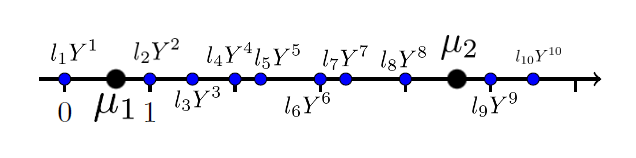
\includegraphics[scale = 0.5]{awdaw}
\end{center}

If we only have one mean to distribute over all $Y^{t_k}$, then the best choice is the weighted mean
%
\[ \mu = \frac{\sum_{k = 1}^m l_k Y^{t_k}}{\sum_{k = 1}^m l_k} \]
%

obtained by differentiating (1) with respect to $\mu$, and simplifying the formula. Now suppose $\mu_1 < \mu_2 < \dots < \mu_K$ is the optimal solution to our problem. If we remove $\mu_K$, then $\mu_1 < \dots < \mu_{K-1}$ is the optimal solution to the subproblem of distributing $K-1$ means among the subset of points who's closest mean is not $\mu_K$ (for otherwise we can move these means to improve our current solution). The optimal choice of $\mu_K$ then becomes the weighted mean of points who are close to $\mu_K$ as possible. Dynamic programming arises from optimal substructure, and we obtain the simple recurrence: If we let $L(m,k)$ be the optimum cost of putting $k$ of the $\mu_i$ in the range $\{ t_1, \dots, t_m \}$, then we may choose an interval $\{ t_p, \dots, t_m \}$ for which $\mu_k$ will be the closest estimate, and then we optimize over $\{ t_1, \dots, t_p \}$ with one less estimate. Our reccurence is

%
\begin{align*}
    L(m,k) = \min_{k \leq p < m} \bigg\{ L(p,k-1) + \frac{\sum_{j = p+1}^m l_j Y^{t_j}}{\sum_{j = p+1}^m l_j} \bigg\}
\end{align*}
%
\[ L(m,1) = \frac{\sum_{j = 1}^m l_j Y^{t_j}}{\sum_{j = 1}^m l_j} \]
%

If we calculate the weighted mean over time, then we may calculate the recurrence in $O(M^3)$ time. In one swoop, we may recursively calculate the means in quadratic time, reducing the asymptotics to $O(M^2)$. By keeping track of the location of the last means recursively, we can build up the optimal choice of means, and reconstruct our data for use in our neural network.

% We thank Zachary Friggstadt for helping optimize the l_1 norm version of the problem.

\subsection{Evaluation}
To compare our methods with each other and with existing approaches, we focus on two questions.\\
1. How well did we identify which devices were active in each time step?\\
2. How well did we identify the single devices consumption?\\
To address the first question we use the F1-Score, ensuring our results are comparable to the works in the section \textit{Literature}. The 
advantage of the F1-Score is that it combines recall and precision and so avoids contortions, which would arise by considering only one of them. For example, assuming we 
identify the refrigerator being active in all time steps we get a optimal recall value, but a low precision, whereas we get a optimal precision by identifying the refrigerator never as active.
\[ \textrm{Precision} = \frac{\textrm{Number of true positive elements}}{\textrm{Number of elements identified as positives}}  \]
\[ \textrm{Recall} = \frac{\textrm{Number of true positives}}{\textrm{Number of elements that are indeed positive}}  \]
\[ \textrm{F1-Score} = \frac{2 \cdot \textrm{Precision} \cdot \textrm{Recall}}{\textrm{Precision} + \textrm{Recall}}\]
For the second question we are interested in the error per timestep. Therefore we
compare the disaggregated energy consumptions per device with the actual device's consumption we have from the REDD
dataset. 
To weight bigger deviations higher than smaller ones, we square the differences and use the root mean squared error instead of the mean squared error to stay within the same unit and thereby comparable. Since we are interested in the error over all devices and timesteps we average over the number of devices and the length of our timeseries
\[\textrm{RMSE} = \sqrt{\frac{\sum^{T}_{t=1}\sum^{N}_{n=1}(\hat{y}^{(n)}_t-y^{(n)}_t)^2}{T \cdot n}} .  \]



\subsection{Implementation}
Our NILM and pre-processing implementations were written in Python, and are publicly available in our \href{https://github.com/CMPUT-466-551-ML-Project/NILM-Project}{NILM-Project} repository.

After choosing which devices from each home we wanted to train our networks against, we removed the contribution of all other devices present in the home from each home's aggregated power time-series.
We chose this approach, instead of generating new aggregated data by taking the sum of the power signal of the chosen devices from each home, in order to preserve the noise present in the aggregated power time-series.
This noise is present even when no recorded device in the home is active, and therefore needed to be preserved so that our networks could account for it during training.

The original data we used had some periods of missing data, and not all devices were sampled at the same frequency.
To overcome this, we padded our time-series data to be fully aligned across all devices and the aggregate recording.
Any missing sample period of less than 600 seconds was padded with the most-recently recorded power value.
Any missing sample period of more than 600 seconds was thrown out.
We used this padded data for training and evaluation.

In order to recover the binary on-off indicators for each device from the power signal, we use a simple thesholding algorithm.
If the power signal is over the threshold, we say that the device is on, and if the power signal is below the threshold, we say that the device is off.
In our implementation, we used a base threshold of 25W across all devices, to account for noise present in the signal.

Our pre-processing algorithms use these recovered binary on-off indicators, along with the padded aggregated data of each home, in order to generate an approximation of the device power usage for use when training our networks.

We implemented our neural networks using the Keras library \cite{Keras}.
Keras is built on top of the Theano library \cite{Theano, Theano2}.
Our network weights were initialized randomly from a uniform distribution.
All experiments described in this paper were trained end-to-end from the random initialization.
The input size of each network was chosen as the average activation length of the device the network was trained against.
The input size was bounded to a maximum 1500 seconds, due to memory constraints on the machines the networks were trained on.

\section{Results}

%TODO: Ensure say that trained on first 4/5 of data, ran on last fifth -> How would be used in real world. Didn't do any CV stuff
% And didnt use devices where they had less than 1000 seconds active (16minutes) for training or test

%TODO: Add reference to the table, correctly
To first get a baseline, we trained and evaluated the auto encoder using the true device signatures to see, at best, how well it should do.
These results are in Table-\ref{tab:RawEstimate}, and highlights how the network does very badly for most of the devices.

We believe that some of the issues with the network are due to not enough training data being available with an adequate amount of device activations for the network to learn on.
To verify this hypothesis, we generated additional synthetic device data and re-trained our networks.
The synthetic device data was generated with the following algorithm:

For each period of time where the device is off, randomly select a real device activation.
With 50-50 chance, apply the activation by adding its power consumption to both the aggregate and device power signals.
We then move ahead in the timeseries by the size of the chosen activation, repeating this procedure while we are still inside the off-period of the device.

This algorithm has the effect of adding many more device activations to the training data.
In addition to training on synthetic data, we preserve the original aggregate and device power signals, which are also used during training.
After testing against the hold-out set, this method seems promising, with our networks being better able to differentiate against the device being on versus being off.
There are still some issues with this approach, such as the network predicting a large constant power consumption when a device is turned off, and being insensitive to some of the same devices as the original network.
However, after adjusting for this constant power off-set, we see performance increases on the NILM task.
This leads us to believe that training on larger datasets or investigating better data synthesis algorithms are likely to lead to improvements in the network's performance.
The results after training with synthetic data are in Table-\ref{tab:RawEstimateAfterGenerate}.

\begin{table*}[t]
	\centering
	$$\begin{tabular}{c||c|c|c|c|c|}
	Device & Total RMSE & f\_score & \% time active& Activation RMSE & Maximum Energy usage \\
	\hline
	Kitchen Outlets & 71.781 & 0.6087 & 72.2\% & 79.489  & 1582.0  \\ % Is house 3 channel 7
	\hline
	Washer \& Dryer  & 209.3 & 0.233 & 1.4\% & 1657.61  & 3222.5 \\ % Is house 1 channel 20
	\hline
	Oven & 165.001 & N/A & 1.2\% & 1500.33  & 1710.0  \\ % Is house 1 channel 3
	\hline
	Lighting & 91.739 & 0.6547 & 78.6\% & 97.199  & 2246.0  \\ % Is house 2 channel 9
	\hline
	\end{tabular}$$
	
	\captionof{table}{Auto Encoder Performance With True Device Signatures} \label{tab:RawEstimate} 
\end{table*}

\begin{table*}[t]
	\centering
	$$\begin{tabular}{c||c|c|c|c|c|}
	Device & Total RMSE & f\_score & \% active & Activation RMSE & Maximum Energy usage\\
	\hline
	Kitchen Outlets & 71.145 & 0.6087 & 72.2\% & 76.398 & 1582.0  \\ % Is house 3 channel 7
	\hline
	Washer \& Dryer & 566.0  & 0.02160  & 1.4\% & 1357.28 & 3222.5  \\ % Is house 1 channel 20
	\hline
	Oven & 287.830 & 0.0196 & 1.2\% & 1103.43 & 1710.0  \\ % Is house 1 channel 3
	\hline
	Lighting & 91.181 & 0.6547 & 78.6\% & 95.631  & 2246.0  \\ % Is house 2 channel 9
	\hline
	\end{tabular}$$
	
	\captionof{table}{Auto Encoder Performance With True Device Signatures, synthetic data} \label{tab:RawEstimateAfterGenerate} 
\end{table*}

Next, we compared the error for the different preprocessing steps in two different ways.
In Table-\ref{tab:PreproccesVsRawNetworkError} we compared how the network did using the device signatures from different preprocessing algorithms versus if it had the true device signature.
In Table-\ref{tab:PreprocessVsRawRMSE}, we then compared the device signature generated by each preprocessing versus the true device signature.
For this table, we can assume that the lower the RMSE, the better the preprocessing.

\begin{table*}[t]
	\centering
	
	$$\begin{tabular}{c||c|c|c|c|c|c|c|}
	Method & Best RMSE & Worst RMSE & Best f\_score & Worst f\_score & Mean RMSE & Mean f\_score & \% Kept\\
	\hline
	Constant & 0.9377 & 2.4089 & 1.495 & 0.6011 & 1.1266 & 1.0329 & 100\% \\
	\hline
	Interval & 0.9595 & 1.7014 & 1.0007 & 0.0054 & 1.087 & 0.7448 & 93.75\% \\
	\hline
	Edge & 0.8587 & 1.2323 & 1.2325 & 0.2141 & 1.0384 & 0.7698 & 56.25\%  \\
	\hline
	Markov & 0.9531 & 1.2217 & 0.7199 & 0.3015 & 1.061 & 0.4769 & 100\%  \\
	\hline
	\end{tabular}$$
	
	\captionof{table}{Preprocessing Relative to Original over All Data} \label{tab:PreproccesVsRawNetworkError} 
\end{table*}


\begin{table*}[t]
	\centering
	
%Label: Methods comparison vs training relative to training with raw data. Over part of data
$$\begin{tabular}{c||c|}
Method & Average RMSE\\
\hline
Constant & 91.5489\\
\hline
Interval & 93.1732 \\
\hline
Edge & 88.9079 \\
\hline
Markov & 90.9915 \\
\hline
\end{tabular}$$
\captionof{table}{RMSE of Preprocessed Generated Signature vs Actual} \label{tab:PreprocessVsRawRMSE}
\end{table*}


\section{Discussion}

For many devices, the neural network will guess approximately constant value rather than accounting for the device being on or off.
This causes the overall estimation to perform badly with precision which causes a low f\_score, a example is in Figure-\ref{fig:KitchenOutlets}, how the estimate and synthesized estimate are essentially constant.
This causes some of the devices, like the Oven, to not even have a f\_score, due to it never estimating a energy usage high enough to be counted as the device being on.

We hypothesize that this occurs due to not having enough examples where the device was on for training. In Figure-\ref{fig:WasherDryer}, the synthesized estimate does much better, with it correctly estimating where the Washer \& Dryer were not on.

For the different preprocessing algorithms, it does not appear that one is far better than the others. The Edge method does very well in general, with its RMSE when running the neural network being only 1.03 times higher on average, and it also produces the device signature that is closest to the true signature. However, it does not always correctly identify that a device is running, with it incorrectly saying that 43.75\% of devices we tested it with did not have any energy usage.

In the cases where the Edge method were to say that a device had no energy signature, one possible solution to avoid this misidentification would be to then use the Markov method to check if the device actually doesn't have any activations, since the Markov method accurately determined if a device used power for all of the examples, and it performed the second best on relative Mean RMSE for the networks, and the second closest device signature to actual signature.

\begin{figure}

\pgfplotsset{legend style={line width=1pt}}
\begin{tikzpicture}[y=.2cm, x=.7cm,font=\sffamily]
\begin{axis}[
xlabel={Time (s)},
ylabel={Power (W)},
legend entries={true,estimate, synthesized estimate, constant synthesized},
legend style={at={(1.00,0.99)},draw=none,fill=none},
]

\addplot+[sharp plot, no marks, thick]
table 
{kitchen_outlets_actual.dat};
\addplot+[sharp plot, no marks, thick]
table 
{kitchen_outlets_estimate.dat};
\addplot+[sharp plot, no marks, thick]
table 
{kitchen_outlets_synthesized_estimate.dat};
\addplot+[sharp plot, no marks, thick]
table 
{kitchen_outlets_constant_synthesized_estimate.dat};
\end{axis}
\end{tikzpicture}

\captionof{figure}{Energy Estimation for Kitchen Outlets}  \label{fig:KitchenOutlets}
\end{figure}

\begin{figure}
%TODO: Move legend, but to where? :O
\pgfplotsset{legend style={line width=0pt, fill=white, fill opacity=0.75, text opacity =1,draw=none,at={(0.99,0.99)}}}
\begin{tikzpicture}[y=.2cm, x=.7cm,font=\sffamily]
\begin{axis}[
xlabel={Time (s)},
ylabel={Power (W)},
legend entries={true,estimate, synthesized estimate, constant synthesized},
%legend style={at={(0.75,1.03)},anchor=south},
]

\addplot+[sharp plot, no marks, thick]
table 
{washer_dryer_actual.dat};
\addplot+[sharp plot, no marks, thick]
table 
{washer_dryer_estimate.dat};
\addplot+[sharp plot, no marks, thick]
table 
{washer_dryer_synthesized_estimate.dat};
\addplot+[sharp plot, no marks, thick]
table 
{washer_dryer_constant_synthesized_estimate.dat};
\end{axis}
\end{tikzpicture}
\captionof{figure}{Energy Estimation for Washer \& Dryer}  \label{fig:WasherDryer}
\end{figure}

\subsection{Future Work}
The simplest direction for future work is to continue to tweak the current network, and see how well it does when trained against a larger dataset.
One potential dataset is UK-DALE \cite{Kelly2}, which measures the power usage from 5 homes with a duration up to 655 days, which is much longer than REDD \cite{Redd}, which was measured over approximately 14 days.
Additionally, investigation into improved data synthesis algorithms or generative models are likely to yield performance increases, by allowing us to generate additional data for the network to train on, potentially targeting scenarios of device usage which did not occur in the dataset.

Another possible extension to this project would be to add more information to the input of the neural network, such as the time of day and day of the week of the input window since certain appliances are more likely to be activated at certain times. Another option would be to find a way to include the information of what the mean of the input window was while still standardizing each input window by subtracting its mean\cite{Kelly}, perhaps by standardizing the power consumption used as the input and then adding the mean as a single number at the end of the input. However, it is not easy to see where the best place to insert this information into the denoising autoencoder architecture would be. Some experimentation would likely be necessary to find an architecture that made effective use of the new information.

As mentioned earlier, generative models such as hidden Markov models seem to be the state-of-the-art for the NILM task \cite{Kolter}\cite{Parson}.
Hidden Markov models would allow us to intuitively model changing device states over time, and would also be useful for generating additional synthetic training data.
Due to time constraints, we were unable to also investigate how well these models perform given our pre-processed device power consumptions.
This avenue of research is still completely open, and seems likely to yield good results.

% Generate the bibliography.

\bibliography{biblio}
\bibliographystyle{plain}

\end{document}
